\documentclass[a4paper, 12pt]{report}
\setlength{\parskip}{0.5em}

\usepackage{graphicx}
\usepackage[vietnamese]{babel}
\usepackage[utf8]{inputenc}
\usepackage{amsmath, amssymb}
\usepackage[top=2cm, bottom=2cm, left=2.5cm, right=2.5cm]{geometry}
\usepackage{titlesec}
\usepackage[many]{tcolorbox}
\usepackage{enumitem}
\usepackage{subcaption}
\usepackage{float}
\usepackage[hidelinks]{hyperref}
\usepackage{pgfplots}
\usepackage{tocloft}
\usepackage{minted}
\usepackage{tabularx}
\usepackage[table,xcdraw]{xcolor}
\usepackage{listings}
\usepackage{tikz}
\usetikzlibrary{positioning}
\usetikzlibrary{shapes,arrows}

\hypersetup{
    colorlinks,
    linkcolor={black!50!black},
    citecolor={blue!50!black},
    urlcolor={blue!80!black}
}


\title{Báo cáo BTL CSDL}
\author{Lâm Đức Anh}
\date{December 2024}

\newcommand{\chapnumfont}{%     % define font for chapter number
  \usefont{T1}{pnc}{b}{n}%      % choose New Chancery, bold, normal shape
  \fontsize{75}{75}%          % font size 100pt, baselineskip 100pt
  \selectfont%                  % activate font
}
\colorlet{chapnumcol}{gray!100}  % color for chapter number

\titleformat{\chapter}[display]
{\filleft\bfseries}
{\filleft\chapnumfont\textcolor{chapnumcol}{\thechapter}}
{-24pt}
{\Huge}

\setlength{\cftchapnumwidth}{3em}
\setlength{\cftbeforechapskip}{2.5em} 
\setlength{\cftbeforesecskip}{0.75em}
\setlength{\cftbeforesubsecskip}{0.5em}



\renewcommand{\thechapter}{\Roman{chapter}}
\renewcommand{\thesection}{\arabic{section}}
% \renewcommand{\thesubsection}{\alph{subsection}.}



\begin{document}


\begin{titlepage}

    \begin{center}

        % Phần trên cùng
        \textbf{\large Đại học Quốc gia Hà Nội}\\[0.2cm]
        \textbf{\large Trường Đại học Công nghệ}\\[2cm]

        \includegraphics[width=0.2\textwidth]{images/UET logo.pdf}\\[3cm]

        % Phần ở giữa
        \textbf{\huge BÁO CÁO ĐỀ TÀI}\\[0.5cm]
        % \textbf{\Large Bài tập lớn Cơ sở dữ liệu}\\[2cm]

        \textbf{\Large Giám sát giao thông trong thời gian thực \\ sử dụng các công nghệ dữ liệu lớn và học sâu}\\[2cm]

        \begin{align*}
            &\textbf{Môn học}:&\text{Kỹ thuật và Công nghệ Dữ liệu lớn}\\
            &\textbf{Giảng viên}:&\text{TS. Trần Hồng Việt}\\[1cm]
            &\textbf{Thành viên nhóm} &\textbf{Mã sinh viên} \\
            &\text{Lâm Đức Anh} &23020326 \\
            &\text{Nguyễn Văn A} &23020000 \\
        \end{align*}
        
        
    \end{center}
    \vfill
    \begin{center}
        \textbf{\large Hà Nội, 2025}
    \end{center}
    
\end{titlepage}

\tableofcontents % Tạo mục lục

\renewcommand{\listfigurename}{Danh mục hình ảnh} % tùy chỉnh tiêu đề
\cleardoublepage
\phantomsection
\addcontentsline{toc}{chapter}{\listfigurename}
\listoffigures

\newpage % Sang trang mới sau mục lục

\chapter{Giới thiệu}

\section{Giới thiệu đề tài}


Ngày nay, bùng nổ dân số và xu hướng đô đô thị hóa nhanh, dân số tập trung đông tại các thành phố lớn
đòi hỏi yêu cầu phát triển cơ sở hạ tầng giao thông để đảm bảo đô thị được vận hành hiệu quả.
Khi hệ thống giao thông ngày càng mở rộng và phát triển, thì các nhà quy hoạch và quản lý đô thị càng quan tâm 
tới bài toán giám sát một mạng lưới giao thông phức tạp của thành phố, đảm bảo cho hệ thống phải an toàn và thông suốt.
Các tình huống thường gặp trên đường bao gồm ùn tắc giao thông, vượt đèn đỏ, lái xe quá tốc độ dẫn đến tai nạn và
không đội mũ bảo hiểm với xe máy và thậm chí là truy vết tội phạm đang tham gia giao thông.
Do đó, giám sát giao thông là một bài toán cơ bản, quan trọng và không thể thiếu với các đô thị lớn nhằm đảm bảo giao thông được vận hành hiệu quả.

\begin{figure}[H]
    \centering
    \includegraphics[width=0.75\textwidth]{images/CCTV.jpg}
    \caption[Camera giám sát trên đường Vành đai 3 Hà Nội]{Camera giám sát trên đường Vành đai 3, Hà Nội. Hiện nay, thành phố Hà Nội triển khai các camera giám sát trên diện rộng hướng đến mục tiêu giám sát giao thông tự động toàn thành phố.}
    \label{fig:traffic}
\end{figure}

Trong một thời gian rất dài trước đây, tại những thành phố lớn, việc giám sát giao thông chủ yếu dựa vào
lực lượng chức năng túc trực trên các tuyến đường và nút giao thông trọng điểm để quan sát, phát hiện và xử lý vi phạm.
Cách tiệp cận truyền thống này phụ thuộc lớn vào số lượng nhân lực và khó đảm bảo khả năng theo dõi trên toàn bộ đô thị.
Tại Việt Nam, từ lâu chính quyền đã cho lắp đặt camera an ninh ở một vài vị trí để theo dõi tình hình giao thông.
Tuy nhiên, việc lắp đặt các camera giám sát một cách có có hệ thống cho việc giám sát tự động chỉ mới được triển khai trong những năm gần đây,
hướng đến mục tiêu giám sát tự động và ra quyết định theo thời gian thực.
Tuy vậy, triển khai giám sát bằng camera trên diện rộng đặt ra nhiều vấn đề và thách thức, trong đó có vấn đề về xử lý
lượng dữ liệu lớn và liên tục trong thời gian thực, có thể gây tắc nghẽn cho hệ thống và làm sai lệch kết quả giám sát.

\begin{figure}[H]
    \centering
    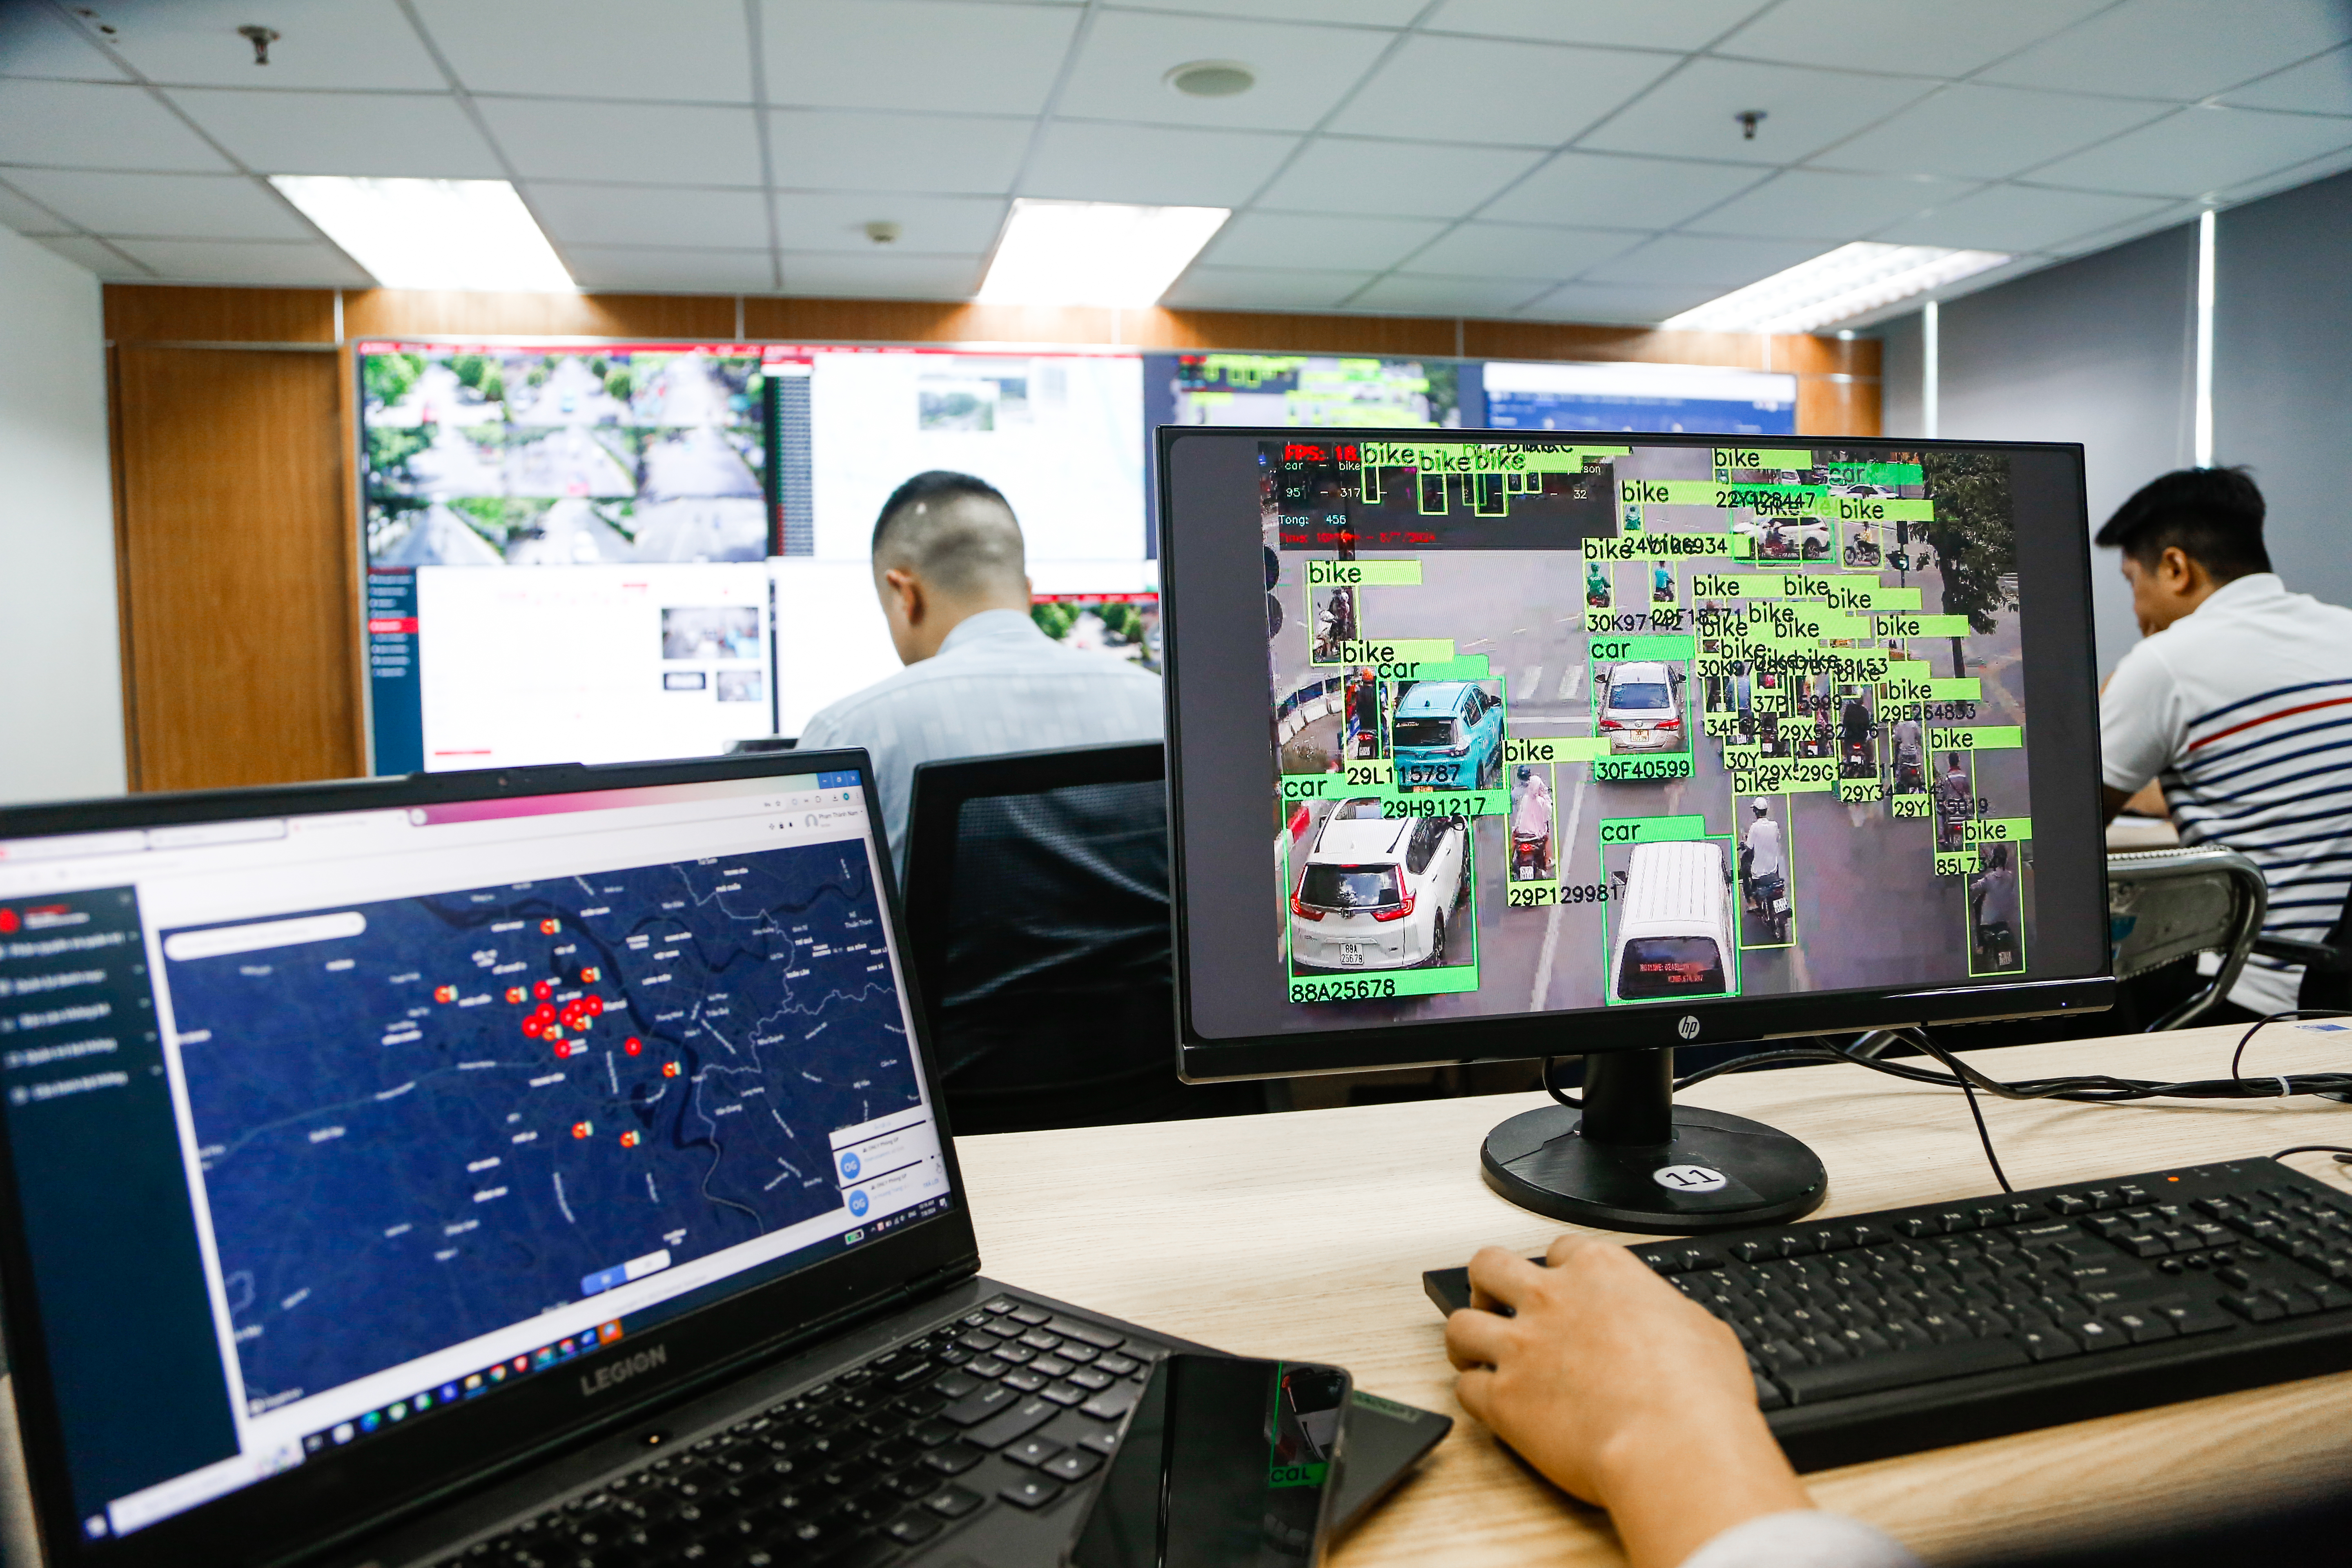
\includegraphics[width=0.85\textwidth]{images/TrungTamDieuHanhHaNoi.png}
    \caption[Trung tâm Điều hành giao thông thông minh Hà Nội]{Bên trong Trung tâm Điều hành giao thông thông minh tại Thành phố Hà Nội, một cán bộ đang theo dõi các phương tiện trên màn hình máy tính.}
    \label{fig:MonitorCentral}
\end{figure}

Trong lĩnh vực Học sâu và Thị giác máy tính, mô hình YOLO là một trong những mô hình tiên tiến cho bài toán nhận diện cũng như theo dõi vật thể trong thời gian thực,
có thể được áp dung trong các bài toán giám sát giao thông như nhận diện biển số xe, phát hiện vượt đèn đò hoặc chạy vượt quá tốc độ, phát hiện không đội mũ khi đi xe máy,
cũng như đếm lưu lượng phương tiện để cảnh báo ùn tắc.
Với một lượng dữ liệu lớn cần xử lý trong thời gian thực, ta có các công nghệ dữ liệu lớn như Apache Kafka kết hợp với Apache Flink
cung cấp nền tảng xử lý thời gian thực với độ trễ thấp, khả năng mở rộng quy mô và khả năng chịu lỗi cao. Khối lượng dữ liệu lớn đó có thể được lưu trữ và truy vấn hiệu quả
thông qua MongoDB, một cơ sở dữ liệu NoSQL được sử dụng nhờ tính linh hoạt với dữ liệu phi cấu trúc.

\newpage
\section{Phát biểu bài toán}

Bài toán ``Giám sát giao thông thời gian thực sử dụng công nghệ dữ liệu lớn và học sâu'' được phát biểu như sau:

\begin{enumerate}
    \item \textit{Đầu vào}: Là một dữ liệu video/hình ảnh được thu thập từ camera giám sát giao thông trên các tuyến đường hoặc tại nút giao, có chứa các phương tiện đang di chuyển trên đường.
    Các video/hình ảnh có độ phân giải và điều kiện quay chụp khác nhau, và đều được truyền phát liên tục từng khung hình trong thời gian thực.
    \item \textit{Đầu ra}: Nhật ký thông tin các phương tiện di chuyển qua đoạn đường, bao gồm biển số xe, ngày giờ di chuyển, các lỗi vi phạm; Báo cáo tình trạng giao thông trên mỗi tuyến đường/nút giao mà camera truyền phát đến.
    \item \textit{Yêu cầu}: Sử dụng các mô hình học sâu để thực hiện các bài toán theo dõi và nhận diện vật thể một cách chính xác; 
    Tích hợp các công nghệ dữ liệu lớn để xử lý song song, phân tán các khung hình nhằm xử lý dữ liệu theo thời gian thực;
    Lưu trữ các thông tin đã qua nhận diện hoặc xử lý vào cơ sở dữ liệu để sẵn dùng cho các tác vụ khác.
\end{enumerate}

Bài toán này có thể được phát biểu theo nhiều cách khác nhau, nhưng chúng tôi sẽ lấy phát biểu trên làm cơ sở để tiến hành quá trình tìm hiểu và nghiên cứu các giải pháp liên quan.
Phạm vi và mục tiêu nghiên cứu sẽ được trình bày cụ thể hơn ở phần sau. 



\section{Các nghiên cứu liên quan}

Trong nhiều năm qua, giám sát giao thông đã trở thành một trong những bài toán nghiên cứu và ứng dụng quan trọng góp phần hỗ trợ và thúc đẩy phát triển các thành phố thông minh, hiện đại.
Trong số đó, có nhiều công trình nghiên cứu không chỉ các thuật toán phát hiện mà còn khai thác các nền tảng tính toán phân tán và công nghệ dữ liệu lớn
để xây dựng hệ thống giám sát thời gian thực.
Chúng tôi đã thực hiện thu thập và phân tích một cách có hệ thống nhiều công trình nghiên cứu liên quan, tập trung vào bài toán chính giám sát giao thông và các bài toán cấu thành bao gồm
nhận dạng biển số xe, phát hiện vi phạm giao thông, ước lượng mật độ giao thông và xây dựng hệ thống xử lý dữ liệu lớn trong thời gian thực.

Bài toán xử lý dữ liệu giao thông thời gian thực sử dụng Apache Kafka và Flink đã được khám phá trong công trình của Gnana Deepthi và cộng sự (2023) \cite{Deepthi2024}. 
Các tác giả đề xuất kiến trúc FRTSPS (Flexible Real-Time Traffic Stream Processing System), cho phép xử lý đồng thời dữ liệu theo lô (batch processing) và dữ liệu theo luồng (stream processing) từ các camera giao thông. 
Kiến trúc này giúp giảm độ trễ và tăng khả năng mở rộng, với Kafka đóng vai trò là bộ đệm dữ liệu đầu vào để quản lý luồng dữ liệu liên tục từ nguồn như camera. 
Sau đó, Flink thực hiện các phép biến đổi như map, filter hay reduce để phân tích các chỉ số như lưu lượng xe, tốc độ trung bình và vị trí phương tiện tại các khoảng thời gian cụ thể. 
Thực nghiệm cho thấy FRTSPS có độ trễ thấp hơn so với các nền tảng như Apache Spark hay Storm. 
Công trình này cho thấy khả năng của Flink trong xử lý dữ liệu giao thông, gợi ý rằng nó có thể áp dụng để phát triển hệ thống giám sát giao thông thông minh tại các đô thị lớn.

\section{Mục tiêu và phạm vi dự án}

\subsection{Mục tiêu dự án}

Mục tiêu tổng quát của đề tài ``Giám sát giao thông thời gian thực sử dụng công nghệ dữ liệu lớn và học sâu'' là xây dựng một hệ thống có khả năng giám sát giao thông tự động
thông qua hệ thống các thiết bị biên. Hệ thống phải có khả năng hoạt động với lượng dữ liệu lớn, nhiều nguồn, hoạt động liên tục trong thời gian thực với độ trễ chấp nhận được,
trong đó được áp dụng hay tích hợp các công nghệ về xử lý dữ liệu lớn và học sâu.
Từ đó cung cấp một giải pháp cơ bản hỗ trợ các cơ quan chức năng trong việc giám sát giao thông tự động.


Mục tiêu cụ thể của dự án này là xây dựng một hệ thống giám sát giao thông tự động dựa trên một hệ thống nhiều camera khác nhau, có khả năng theo dõi các phương tiện,
phát hiện các vi phạm (nếu có), phân tích tình trạng giao thông với dữ liệu được gửi liên tục từ hệ thống camera đó trong thời gian thực. Trong đó:

\begin{itemize}
    \item \textit{Xử lý dữ liệu luồng theo thời gian thực}: Tích hợp Apache Kafka để thu thập và truyền phát dữ liệu liên tục theo thời gian thực, với khả năng truyền phát thông tin liên tục từ nhiều nguồn khác nhau cùng lúc;
    Sử dụng Apache Flink để xử lý dữ liệu luồng thời gian thực với hiệu suất cao và khả năng mở rộng dễ dàng khi lượng dữ liệu tăng cao.
    \item \textit{Huấn luyện mô hình học sâu}: Huấn luyện, triển khai mô hình YOLO cùng các thuật toán tracking cho việc theo dõi chuyển động của các phương tiện, phân tích tình trạng giao thông với tốc độ xử lý nhanh; 
    Huấn luyện, triển khai mô hình CNN sâu và các thuật toán khác để nhận diện biển kí tự biển số xe và nhận diện các lỗi vi phạm với độ chính xác cao.
    
    \item \textit{Lưu trữ dữ liệu}: Lưu trữ các kết quả sau khi đã nhận diện, phân tích vào MongoDB, giúp quản lý và truy xuất thông tin giao thông về sau dễ dàng và hiệu quả.
    
\end{itemize}



\subsection{Phạm vi thực hiện}

Do luôn tồn tại sự cản trở tự nhiên về mặt địa lý, giới hạn về dữ liệu và tài nguyên tính toán, nên mục này đặt ra một số phạm vi hoặc giới hạn hiện có trong dự án này.

Về dữ liệu đầu vào:

\begin{itemize}
    \item Video đường phố hoặc ngã tư, được ghi hình theo thời gian thực bởi camera, tập trung chủ yếu vào giao thông trong đô thị tại Việt Nam.
    \item  
\end{itemize}

Công nghệ và công cụ sử dụng:
\begin{itemize}
    \item Ngôn ngữ chính: Python
    \item Xử lý ảnh và học sâu: OpenCV, Ultralytics, PyTorch.
    \item Xử lý dữ liệu: Apache Kafka, Apache Flink, MongoDB.
    \item Môi trường triển khai: Docker, WSL Ubuntu.
\end{itemize}

Giới hạn nghiên cứu:
\begin{itemize}
    \item Nghiên cứu tập trung vào bài toán xử lý luồng dữ liệu trong thời gian thực, chưa tập trung vào xây dựng mô hình học sâu tối ưu cho bài toán.
    \item Nghiên cứu dừng lại ở một hệ thống thực hiện xử lý luồng dữ liệu từ lúc nó được sinh ra ở camera cho tới khi đến được trình giám sát và lưu vào cơ sở dữ liệu, chưa tích hợp vào một hệ thống quản lý giao thông lớn hơn.
    \item Nghiên cứu chưa mở rộng sang các thiết bị biên khác, chưa mở rộng đối với giao thông nước ngoài.
\end{itemize}

Với phạm vi thực hiện này, đề tài hướng đấy xây dựng một hệ thống giám sát giao thông có thể xử lý một luồng dữ liệu lớn trong thời gian, với độ tin cậy và khả năng chịu lỗi cao,
đồng thời áp dụng các mô hình học sâu cho từng bài toán, đảm bảo tính ứng dụng cao trong thực tế.

\section{Phương pháp thực hiện}

\subsection{Phương pháp nghiên cứu lý thuyết}

Tìm hiểu và tổng hợp các nghiên cứu liên quan đến bài toán giám sát giao thông tự động trong thành phố, đặc biệt là các phương pháp sử dụng các công nghệ dữ liệu lớn.

Tìm hiểu các thuật toán, mô hình học sâu để giải quyết các bài toán con của giám sát giao thông.

Nghiên cứu các công nghệ xử lý dữ liệu lớn như Apache Kafka, Apache Flink, MongoDB để đảm bảo hệ thống có khả năng hoạt động với dữ liệu luồng theo thời gian thực.

\subsection{Phương pháp triển khai}

\subsection{Phương pháp thực nghiệm và đánh giá}





\chapter{Cơ sở lý thuyết}

\section{Bài toán giám sát giao thông}

\subsection{Tổng quan về giám sát giao thông}

Giám sát giao thông (Traffic Monitoring) trong thành phố là việc thu thập các dữ liệu về giao thông, sau đó tiến hành phân tích 
và đưa ra các quyết định tác động trở lại giao thông như cảnh báo, điều tiết hoặc ngăn chặn, nhằm giữ cho giao thông được vận hành thông suốt và trật tự.
Ngày nay, với sự tiến bộ về công nghệ, bài toán giám sát giao thông tự động là việc thu thập dữ liệu từ hệ thống thiết bị biên như camera, cảm biến IoT,
sau đó phân tích và xử lý tự động bằng AI và thuật toán để phát hiện sự kiện, gợi ý hành động và hiển thị thông tin thời gian thực cho người giám sát.

Các hệ thống hiện đại giải quyết bài toán giám sát giao thông tự động hiện nay chủ yếu xoay quanh 3 thành phần chính: Thiết bị biên, Trung tâm xử lý, Trình giám sát.

\begin{enumerate}
  \item Thiết bị biên: 
  \item Trung tâm xử lý và lưu trữ:
  \item Trình giám sát:
\end{enumerate}

\subsection{Giám sát giao thông với hệ thống camera}

Trong số các loại thiết bị biên, thì camera giám sát hiện là loại thiết bị phổ biến nhất ứng dụng trong giám sát giao thông, bởi tính đơn giản, tiện dụng, dễ lắp đặt, dễ tích hợp.
Đặc điểm của camera là thu thập dữ liệu dưới dạng hình ảnh, vì vậy khi triển khai hệ thống camera trên diện rộng, lượng dữ liệu cần xử lý là rất lớn, vì vậy với hệ thống giám sát giao thông với hệ thống camera,
ta không chỉ quan tâm với việc xử lý dữ liệu sao cho đúng, mà còn cần quan tâm tới việc truyền phát và xử lý dữ liệu như nào để nhanh, hiệu quả nhất. 

\subsection{Các bài toán con}

Giám sát giao thông là một bài toán lớn, tổng quát, có nhiều vấn đề. Các bài toán con tiêu biểu có thể kể đến:

\begin{itemize}
  \item Nhận diện biển số xe:
  \item Nhận diện vượt đèn đỏ:
  \item Nhận diện không đội mũ:
  \item Phân tích tình trạng giao thông:
\end{itemize}

\section{Học sâu}

Học sâu (Deep Learning) là một nhánh của Học máy và Trí tuệ nhân tạo, tập trung vào việc xây dựng và huấn luyện
các mô hình dựa trên mạng nơ-ron nhân tạo. Học sâu mô phỏng cách mà não bộ con người hoạt động qua nhiều lớp nơ-ron,
nó học qua nhiều tầng khác nhau và tự động học được các đặc trưng phức tạp từ dữ liệu đầu vào.
So với các phương pháp học máy truyền thống, học sâu có khả năng xử lý dữ liệu với độ phức tạp cao mà không cần
thiết kế đặc trưng thủ công. Điều này giúp học sâu được ứng dụng rộng rãi trong nhiều lĩnh vực, trong đó có thị giác máy tính.

Với bài toán giám sát giao thông, mô hình học sâu sẽ tự động hóa việc nhận diện phương tiện và phân tích tình trạng giao thông.
Trong phần này, chúng tôi sẽ trình bày chủ yếu về CNN và YOLO, hai mô hình học sâu quan trọng nhất cho bài toán nhận diện vật thể,
cùng các kỹ thuật khác cho việc xử lý các bài toán liên quan.

\subsection{YOLO trong phát hiện phương tiện}

YOLO là một trong những thuật toán phát hiện đối tượng tiên tiến nhất hiện nay, được sử dụng rộng rãi trong nhiều lĩnh vực.


\subsubsection{Kiến trúc của mô hình YOLO}

\subsubsection{Ưu điểm và hạn chế của YOLO}

Ưu điểm: Tốc độ xử lý nhanh; Tính linh hoạt; Dễ dàng triển khai

Hạn chế: Yêu cầu dữ liệu huấn luyện đa dạng; Cần tài nguyên tính toán; Khả năng nhận diện khi vật thể bị che khuất

\subsubsection{Ứng dụng YOLO trong giám sát giao thông}

YOLO có thể ứng dụng để nhận diện các phương tiện đang tham gia giao thông trên đường, nhận diện vị trí biển số của phương tiện, nhận diện ví trí các kí tự trên biển số, nhận diện tín hiệu đèn tại các ngã tư, v.v.

YOLO khi kết hợp với thuật toán SORT có thể thực hiện theo dõi chuyển động của vật thể, từ đó còn có thể ứng dụng vào việc nhận diện các xe vượt đèn đỏ hoặc ước lượng tốc độ xe.

\subsection{CNN cho bài toán phân loại}

CNN là một trong những kiến trúc quan trọng nhất trong lĩnh vực thị giác máy tính.

\subsubsection{Kiến trúc của mô hình CNN}

Kiến trúc của một CNN thường gồm: lớp tích chập, hàm kích hoạt, lớp pooling, lớp fc.

\begin{figure}[H]
    \centering
    \includegraphics[width=1\textwidth]{images/CNN architecture.drawio.pdf}
    \caption[Kiến trúc mô hình CNN]{Kiến trúc mô hình CNN.}
    \label{fig:cnn-architecture}
\end{figure}

\subsubsection{Ứng dụng CNN trong giám sát giao thông}

CNN có thể xác định 

\subsection{Nhận diện kí tự biển số xe}

Nhận diện kí tự biến số xe? Đầu vào, đầu ra?



\subsection{Nhận diện tốc độ xe}

Đầu vào đầu ra? Phương pháp nhận diện tốc độ xe?

\subsection{Nhận diện xe vượt đèn đỏ}

\subsection{Ước lượng mật độ giao thông}


\section{Công nghệ dữ liệu lớn}

\subsection{Apache Kafka}


Apache Kafka là một hệ thống phân tán được xây dựng với mục tiêu truyền phát một lượng dữ liệu rất lớn trong thời gian thực với độ trễ thấp,
đồng thời có khả năng mở rộng cao. Ban đầu Kafka được phát triển bởi LinkedIn, nhưng sau đó được chuyển giao và trở thành dự án mã nguồn mở 
trong hệ sinh thái Apache và nhanh chóng được cộng đồng công nghệ chấp nhận rộng rãi.

Kafka hoạt động dựa trên 3 thành phần chính:

\begin{enumerate}
    \item \textit{Producer} (Bên cung cấp): để chỉ các ứng dụng hay hệ thống nơi dữ liệu được tạo ra và cần được phân phối đến Kafka.
    Mỗi dữ liệu truyền phát đến Kafka sẽ được sắp xếp theo các topic do người dùng lựa chọn, mỗi topic dữ liệu mang ý nghĩa và mục đích riêng,
    phản ánh một luồng dữ liệu cụ thể cần trao đổi trong hệ thống.
    Mỗi topic được chia thành nhiều partition, cho phép Kafka phân tán dữ liệu trên nhiều máy chủ, từ đó tăng khả năng
    xử lý song song và hỗ trợ mở rộng khi khối lượng dữ liệu tăng.

    \item \textit{Consumer} (Bên tiêu thụ): để chỉ các ứng dụng hay hệ thống cần truy cập và sử dụng dữ liệu được Kafka lưu trữ.
    Mỗi consumer sẽ đăng kí các topic mà nó quan tâm, từ đó sẽ nhận tự động luồng dữ liệu mà producer đã gửi vào Kafka.
    Các consumer có thể làm việc độc lập, tức là mỗi consumer sẽ nhận toàn bộ dữ liệu trong topic, hoặc hoạt động theo nhóm,
    khi đó dữ liệu trong topic sẽ được phân phát giữa các consumer trong nhóm để xử lý song song.

    \item \textit{Broker}: là các máy chủ trong hệ thống Kafka, chịu trách nhiệm nhận và lưu trữ dữ liệu từ các producer.
    Mỗi broker quản lý một hoặc nhiều partition của topic. Vì Kafka hỗ trợ tính toán phân tán nên các broker có thể phân phối
    dữ liệu giữa các máy chủ để nâng cao hiệu suất và tăng cường khả năng chịu lỗi.
\end{enumerate}

\begin{figure}[H]
    \centering
    \includegraphics[width=1\textwidth]{images/kafka_flow.pdf}
    \caption[Luồng hoạt động của Apache Kafka]{Luồng hoạt động nhận và gửi tin của Apache Kafka. Các hình tròn đại diện cho các tin nhắn được gửi qua Kafka.}
    \label{fig:kafka-flow}
\end{figure}

Kafka được xem là một thành phần quan trọng trong nhiều hệ thống xử lý dữ liệu lớn hiện nay, nhờ khả năng đáp ứng tốt các yêu cầu
về truyền phát dữ liệu liên tục ở quy mô lớn. Dưới đây là các đặc điểm nổi bật của Kafka:

\begin{itemize}
    \item \textit{Khả năng mở rộng}: Kafka có thể mở rộng để xử lý lượng dữ liệu lớn bằng cách thêm các broker vào cluster. 
    Các partition của topic có thể được phân phối trên nhiều broker, giúp tăng khả năng xử lý đồng thời và cân bằng tải giữa các nút trong hệ thống.
    \item \textit{Tính chịu lỗi cao}: Kafka hỗ trợ cơ chế sao lưu và phân phối dữ liệu, đảm bảo rằng dữ liệu không bị mất khi có sự cố xảy ra. 
    Mỗi partition có thể có một hoặc nhiều bản sao (replica) để bảo vệ dữ liệu khỏi mất mát. 
    Các broker sẽ tự động chuyển đổi sang các bản sao khi một broker gặp sự cố.
    \item \textit{Hiệu suất cao}: Kafka có thể xử lý hàng triệu sự kiện mỗi giây với độ trễ rất thấp. 
    Điều này là nhờ vào việc sử dụng cơ chế write-ahead log (WAL), nơi dữ liệu được ghi vào log trước khi được xử lý. 
    Kafka có khả năng tối ưu hóa việc ghi dữ liệu và xử lý đồng thời, giúp đạt được hiệu suất cao.
    \item \textit{Tính linh hoạt}: Kafka hỗ trợ nhiều kiểu dữ liệu và ứng dụng khác nhau, từ các ứng dụng yêu cầu xử lý thời gian thực 
    (như hệ thống giám sát và phân tích dữ liệu trực tuyến) đến các ứng dụng yêu cầu lưu trữ và phân tích dữ liệu theo thời gian dài (như hệ thống log và dữ liệu lịch sử).
    \item \textit{Tích hợp dễ dàng}: Kafka dễ dàng tích hợp với các công cụ và hệ thống khác trong hệ sinh thái dữ liệu lớn như Apache Spark, Apache Flink, Hadoop, và Elasticsearch. 
    Điều này giúp xây dựng các pipeline xử lý dữ liệu phức tạp mà không gặp phải sự gián đoạn trong quá trình truyền tải dữ liệu.

\end{itemize}

[Thêm một đoạn nữa nói về ứng dụng của Kafka trong xử lý dữ liệu lớn]

\newpage

\subsection{Apache Flink}

Apache Flink là một nền tảng mã nguồn mở mạnh mẽ dùng để xử lý dữ liệu luồng theo thời gian thực và dữ liệu theo lô. 
Khác với các hệ thống xử lý theo mô hình micro-batch, Flink thực hiện xử lý dữ liệu streaming thực sự, 
nghĩa là mỗi bản ghi được xử lý ngay khi xuất hiện, với độ trễ rất thấp và khả năng mở rộng cao.
Flink được thiết kế theo kiến trúc phân tán, cho phép triển khai linh hoạt trên nhiều node trong một cụm máy
và có thể tích hợp linh hoạt với nhiều hệ thống dữ liệu như Kafka, MongoDB hay các hệ quản trị cơ sở dữ liệu khác.

\subsubsection{Kiến trúc và nguyên lý hoạt động}

Apache Flink gồm 3 thành phần chính: JobManager, TaskManager và Client.
\begin{itemize}
  \item \textit{Client}: Chịu trách nhiệm biên dịch và gửi job đến đến cụm máy Flink.
  \item \textit{JobManager}: Thực hiện lập kế hoạch thực thi các job được gửi lên, quản lý luồng dữ liệu, 
  điều phối công việc giữa các node, giám sát quá trình thực thi để đảm bảo toàn bộ công việc được xử lý đúng và hiệu quả.
  \item \textit{TaskManager}: Chịu trách nhiệm thực thi các tác vụ cụ thể, xử lý dữ liệu đầu vào, gửi kết quả đầu ra hoặc kết quả trung gian đến các node khác trong cụm.
\end{itemize}

Flink thực hiện xử lý dữ liệu streaming thực sự, trong đó mỗi bản ghi được xử lý ngay khi đến thay vì gom thành các batch nhỏ như trong micro-batch,
cho phép tiến tới một hệ thống có độ trễ xử lý thấp và xử lý liên tục trong thời gian thực.
Bên cạnh đó, Flink sử dụng cơ chế checkpointing để lưu trạng thái định kỳ, sử dụng state backend để quản lý và truy xuất trạng thái trong quá trình xử lý.
Ngoài ra, Flink còn hỗ trợ xử lý theo thời gian sự kiện kết hợp với watermark, giúp xử lý chính xác các luồng dữ liệu đến trễ hoặc không theo thứ tự. 


Flink có khả năng tích hợp linh hoạt với nhiều công nghệ dữ liệu lớn khác như Apache Kafka, HDFS, MongoDB hoặc Canssandra, cho phép xây dựng các pipeline xử lý dữ liệu phức tạp và mở rộng dễ dàng.
Trong lập trình, Flink cung cấp DataStream API phục vụ xử lý dữ liệu streaming, cho phép người dùng định nghĩa luồng xử lý thông qua các phép biến đổi như map, filter, keyBy, window hoặc aggregation.
Bên cạnh các API bằng Java và Scala, Flink cũng cung cấp API cho Python (PyFlink), hỗ trợ người dùng triển khai và quản lý các ứng dụng xử lý dữ liệu luồng bằng Python,
cho phép mở rộng khả năng tiếp cận và phát triển hệ thống trong nhiều tình huống khác nhau, đặc biệt là khi cần tích hợp với các mô hình học sâu.

\subsubsection{Các ưu điểm của Flink}

\begin{itemize}
  \item \textit{Xử lý dữ liệu thời gian thực với độ trễ thấp}: Độ trễ của Flink rất thấp, chỉ tính bằng mili-giây,
  có thể đáp ứng tốt các yêu cầu phân tích và ra quyết định theo thời gian thực, đặc biệt phù hợp cho các bài toán giám sát theo thời gian thực.
  \item \textit{Xử lý nhất quán và toàn vẹn}: Flink có cơ chế cho phép xử lý dữ liệu dựa trên thời gian sự kiện thay vì thời gian hệ thống, cho phép duy trì tính toàn vẹn của kết quả khi dữ liệu không đồng bộ.
  Flink cũng có các cơ chế đảm bảo tính nhất quán, đảm bảo mỗi bản ghi được xử lý duy nhất một lần ngay cả khi gặp sự cố.
  \item \textit{Khả năng tích hợp linh hoạt}: Flink hỗ trợ kết nối và trao đổi dữ liệu với nhiều hệ thống phổ biến như Apache Kafka, Cassandra, MongoDB,
  giúp xây dựng pipeline liên tục từ thu thập, xử lý đến lưu trữ. Flink cũng hỗ trợ xuất kết quả sang nhiều định dạng khác nhau, phù hợp cho các hệ thống giám sát hay dashboard.
  \item \textit{Khả năng mở rộng và chịu lỗi cao}: Nhờ kiến trúc phân tán và cơ chế lập lịch linh hoạt, Flink có thể mở rộng quy mô xử lý lên tới hàng trăm node để đáp ứng khối lượng dữ liệu cực lớn.
  Khi có lỗi xảy ra, Flink tự động khôi phục từ các checkpoint gần nhất mà không làm gián đoạn quá trình xử lý. Những điều giúp Flink duy trì hoạt động ổn định trong môi trường thực tế.
\end{itemize}


\subsection{MongoDB}

MongoDB là một hệ quản trị cơ sở dữ liệu NoSQL phổ biến, được thiết kế để lưu trữ và quản lý dữ liệu phi cấu trúc hoặc cấu trúc linh hoạt,
được sử dụng rộng rãi trong các hệ thống yêu cầu khả năng mở rộng và hiệu suất cao.
Khác với hệ quản trị cơ sở dữ liệu quan hệ (RDBMS) sử dụng các bảng và quan hệ, thì MongoDB lưu trữ dưới dạng documents trong collections.
Mỗi document trong MongoDB là một đối tượng JSON (JavaScript Object Notation) hoặc BSON (Binary JSON), cho phép lưu trữ các kiểu dữ liệu phức tạp như mảng, đối lượng lồng nhau hay kiểu dữ liệu thời gian.

\begin{figure}[ht]
\centering
\begin{minipage}{0.85\linewidth}
\begin{verbatim}
{
  "timestamp": "2025-11-07T14:23:10Z",
  "camera_id": "cam-02-hcm",
  "location": {
    "lat": 10.762622,
    "lon": 106.660172
  },
  "vehicle": {
    "type": "motorbike",
    "plate": "59K1-12345",
    "color": "blue"
  },
  "speed_kmh": 58.4,
  "event": "speeding",
  "confidence": 0.93
}
\end{verbatim}
\end{minipage}
\caption[Cấu trúc dữ liệu trong MongoDB]{Ví dụ cấu trúc dữ liệu trong MongoDB. MongoDB là một cơ sở dữ liệu NoSQL kiểu document, thường được viết theo định dạng JSON.}
\label{fig:json-kafka}
\end{figure}

\subsubsection{Cấu trúc và nguyên lý hoạt động của MongoDB}

Trong MongoDB, dữ liệu được lưu trữ dưới dạng document, mỗi document là một bộ dữ liệu chứa các cặp khóa-giá trị, tương tự như một đối tượng JSON. 
Một document có thể bao gồm nhiều trường với các kiểu dữ liệu khác nhau, từ chuỗi, số, đến mảng hoặc đối tượng lồng nhau. 
Điều này cho phép MongoDB xử lý dữ liệu phức tạp và không cần phải tuân theo một sơ đồ dữ liệu cố định như trong các cơ sở dữ liệu quan hệ.

Các document được nhóm lại thành collections. Một collection có thể chứa nhiều document và không yêu cầu các document phải có cấu trúc giống nhau. 
Điều này mang lại sự linh hoạt rất lớn, vì bạn có thể lưu trữ các loại dữ liệu khác nhau trong cùng một collection mà không cần phải thay đổi cấu trúc của các bảng hay cơ sở dữ liệu như trong hệ quản trị cơ sở dữ liệu quan hệ.

MongoDB sử dụng cơ chế replication để sao lưu và bảo vệ dữ liệu, đảm bảo rằng nếu một nút trong cluster gặp sự cố, dữ liệu vẫn có thể được truy cập thông qua các bản sao (replica set). 
Một replica set là một nhóm các mongod processes (MongoDB processes), trong đó một node được chọn làm primary và các node còn lại là secondary. Dữ liệu được sao chép từ node primary sang các node secondary, giúp duy trì sự đồng nhất và tính sẵn sàng cao.

\subsubsection{Các ưu điểm nổi bật của MongoDB}

MongoDB có một số tính năng nổi bật giúp nó trở thành lựa chọn phổ biến trong việc xử lý và lưu trữ dữ liệu lớn:

\begin{itemize}
    \item Khả năng mở rộng (Scalability): MongoDB hỗ trợ khả năng mở rộng ngang (horizontal scaling) thông qua cơ chế sharding. 
    Sharding cho phép phân chia dữ liệu và lưu trữ nó trên nhiều máy chủ, giúp ứng dụng có thể mở rộng và xử lý một lượng dữ liệu lớn mà không gặp phải sự chậm trễ hoặc giới hạn tài nguyên.
    \item Tình linh hoạt trong cấu trúc dữ liệu: MongoDB không yêu cầu dữ liệu phải tuân theo một schema cố định như trong các hệ quản trị cơ sở dữ liệu quan hệ. 
    Điều này cho phép các ứng dụng thay đổi cấu trúc dữ liệu mà không gặp phải những thay đổi phức tạp trong cấu trúc cơ sở dữ liệu. 
    Mỗi document trong MongoDB có thể có một cấu trúc hoàn toàn khác biệt với các document khác trong cùng một collection.
    \item Hiệu suất cao: MongoDB sử dụng cơ chế in-memory và indexing để tối ưu hóa việc truy vấn dữ liệu. 
    Các chỉ mục (index) có thể được tạo cho bất kỳ trường nào trong một document, giúp giảm thời gian truy vấn và cải thiện hiệu suất khi làm việc với dữ liệu lớn.
    \item Cơ chế sao lưu và phục hồi dữ liệu: MongoDB hỗ trợ cơ chế sao lưu và phục hồi dữ liệu rất mạnh mẽ thông qua replica sets và snapshotting. 
    Các replica set không chỉ giúp tăng tính khả dụng của hệ thống mà còn bảo vệ dữ liệu khỏi bị mất mát trong trường hợp xảy ra sự cố.
    \item Quản lý dữ liệu phi cấu trúc: MongoDB rất phù hợp với các ứng dụng xử lý dữ liệu phi cấu trúc hoặc dữ liệu bán cấu trúc như dữ liệu JSON, XML, log file, dữ liệu web scraping, và dữ liệu cảm biến. 
    Với MongoDB, các nhà phát triển có thể dễ dàng lưu trữ và truy vấn các loại dữ liệu này mà không phải lo lắng về việc thay đổi cấu trúc dữ liệu thường xuyên.

\end{itemize}

\subsubsection{Ứng dụng của MongoDB trong xử lý dữ liệu lớn}

MongoDB đặc biệt hữu ích trong các hệ thống xử lý dữ liệu lớn vì khả năng mở rộng và linh hoạt của nó. 
Trong môi trường dữ liệu lớn, nơi mà lượng dữ liệu có thể phát sinh nhanh chóng và có thể đến từ nhiều nguồn khác nhau, 
MongoDB cung cấp một nền tảng để lưu trữ và truy vấn dữ liệu mà không gặp phải sự chậm trễ hoặc tắc nghẽn. 
Nó có thể được sử dụng trong các ứng dụng web, phân tích dữ liệu lớn, hệ thống lưu trữ log, hệ thống IoT, và các ứng dụng cần xử lý và phân tích dữ liệu thời gian thực.

Một ví dụ điển hình là trong các ứng dụng phân tích log, MongoDB có thể được sử dụng để lưu trữ và truy vấn các tệp log từ nhiều nguồn khác nhau. 
Các công ty công nghệ lớn sử dụng MongoDB để lưu trữ và phân tích dữ liệu nhạy cảm và phi cấu trúc từ các trang web và dịch vụ của họ.

Ngoài ra, MongoDB còn hỗ trợ tích hợp tốt với các công cụ khác trong hệ sinh thái xử lý dữ liệu lớn, chẳng hạn như Apache Flink, để phân tích và xử lý các tập dữ liệu không lồ. 
Khi kết hợp với các công cụ như Kafka và Flink, MongoDB có thể giúp xây dựng các hệ thống phân tích dữ liệu thời gian thực mạnh mẽ, có thể xử lý và phân phối dữ liệu với độ trễ thấp và khả năng mở rộng cao.





\chapter{Phương pháp đề xuất}

\section{Kiến trúc hệ thống}

Hệ thống giám sát giao thông dựa trên công nghệ dữ liệu lớn và học sâu bao gồm 3 thành phần chính:
Thiết bị biên (Edge Devices Layer), Trung tâm dữ liệu và xử lý (Processing and Data Central Layer) và Trình giám sát (Monitoring Layer).

\subsection{Thiết bị biên}

Thiết bị biên là các thiết bị thu nhận hoặc phát sinh dữ liệu trực tiếp tại hiện trường.
Đối với hệ thống giám sát giao thông, thiết bị biên có thể bao gồm các camera giám sát, hệ thống đèn tín hiệu, cảm biến giao thông.
Với quy mô và phạm vi của dự án này, hệ thống các thiết bị biên tương đương với hệ thống các camera giám sát được đặt trên cao,
tại các tuyến đường hoặc nút giao của thành phố.

Tùy vào nhu cầu thực hiện các nhiệm vụ mà các thiết bị biên sẽ có phần cứng phù hợp và các chương trình tính toán được lập trình sẵn.
Dự án này thực hiện với giả sử các camera sẽ có độ phân giải HD, được đặt một góc quay chính diện và phù hợp tại các con đường hoặc nút giao,
có phần cứng phù hợp để tích hợp các chương trình xử lý cơ bản.

Trong hệ thống này, các camera sẽ tiến hành ghi lại các khung hình, xử lý ảnh cơ bản, áp dụng mô hình theo dõi vật thể cơ bản
và tiến hành truyền dữ liệu thời gian thực theo từng khung hình về trung tâm xử lý. Để xử lý dữ liệu streaming theo thời gian thực,
các camera sẽ không gửi trực tiếp đến trung tâm xử lý mà thực hiện gửi dữ liệu đến các topic trong Kafka, giao cho Kafka thực hiện phân phối dữ liệu.




\subsection{Trình giám sát}

Trình giám sát là ứng dụng cuối được sử dụng bởi các giám sát viên. Trong hệ thống giám sát giao thông thời gian thực, trình giám sát là đầu ra của hệ thống, hiển thị được hình ảnh truyền phát từ các camera,
thông báo các sự kiện diễn ra và phân tích tình trạng giao thông, tất cả trong thời gian thực. Trình giám sát sẽ nhận dữ liệu streaming theo thời gian thực mà trung tâm xử lý gửi đến Kafka,
hiển thị trực quan trên màn hình giao diện người dùng.



\subsection{Truyền phát}

Tầng truyền phát là cấu nối trung gian giữa các thiết bị biên, trung tâm xử lý và trình giám sát.
Với hệ thống yêu cầu xử lý dữ liệu lớn thì công việc truyền phát càng quan trọng và có ý nghĩa.
Trong hệ thống giám sát giao thông, dữ liệu được sinh ra liên tục từng khung hình, từng sự kiện (biển số, tốc độ, vi phạm, mật độ,...),
nên hệ thống cần một cơ chế truyền phát liên tục, bền vững, an toàn, chịu tải cao và tránh phụ thuộc giữa các thành phần.
Công việc truyền phát trong hệ thống của chúng tôi sử dụng nền tảng Apache Kafka.

Kafka giao tiếp với cả mặt trước (dữ liệu thô từ camera), phần giữa (dữ liệu xử lý trung gian) và mặt sau (dữ liệu đã xử lý gủi đến trình giám sát và cơ sở dữ liệu) của hệ thống.
Việc truyền phát dữ liệu của Kafka trong hệ thống được minh họa tại Hình \ref{fig:kafka-role}.

\begin{figure}[H]
    \centering
    \includegraphics[width=1\textwidth]{images/Kafka role.pdf}
    \caption[Sơ đồ truyền phát dữ liệu của Kafka trong hệ thống]{Sơ đồ truyền phát dữ liệu của Kafka với các thành phần khác trong hệ thống. Kafka đóng vai trò là nơi nhận phát dữ liệu trong hệ thống giám sát giao thông thời gian thực. }
    \label{fig:kafka-role}
\end{figure}

\newpage
Ở phía thiết bị biên, mỗi camera chỉ thực hiện gửi các khung hình và thông tin đã được xử lý sơ bộ đến Kafka mà không cần kết nối trực tiếp với trung tâm xử lý.
Điều này tách biệt giữa nguồn dữ liệu và quá trình xử lý, mỗi camera có thể hoạt động độc lập và không bị ảnh hưởng bởi trạng thái của các thành phần khác, tránh buộc camera phải kết nối với nhiều dịch vụ khác nhau.
Kafka chịu trách nhiệm thu thập luồng dữ liệu lớn từ nhiều camera cùng lúc, có cơ chế đệm để tránh mất dữ liệu khi hàng đợi bị ùn tắc.


Ở trung tâm xử lý, Apache Flink tiêu thụ dữ liệu streaming từ Kafka để thực hiện các tác vụ phân tích theo thời gian thực.
Kafka giúp Flink có thể mở rộng theo chiều ngang và duy trì khả năng xử lý ổn định ngay cả khi dữ liệu tăng đột biến.
Kafka cũng đảm bảo dữ liệu được phân phối theo đúng thứ tự và có thể phục hồi khi xảy ra sự cố.


Với các dữ liệu đầu ra sau khi xử lý, bao gồm biển số, sự kiện giao thông, kết quả phân tích giao thông, Kafka đảm nhiệm tự động phân phối chúng đến trình giám sát hay cơ sở dữ liệu.
Trình giám sát không cần truy vấn liên tục đến trung tâm xử lý hay cơ sở dữ liệu, vì Kafka đã đẩy luồng dữ liệu trực tiếp theo thời gian thực.
Điều này đảm bảo trình giám sát có thể hiển thị thời gian thực, độ trễ thấp, hoạt động ổn định và không ảnh hưởng lẫn nhau.


\subsection{Xử lý luồng dữ liệu}

\begin{figure}[H]
    \centering
    \includegraphics[width=0.95\textwidth]{images/Flink role.pdf}
    \caption[Sơ đồ luồng dữ liệu trong hệ thống]{Sơ đồ luồng dữ liệu đi trong hệ thống. Apache Flink ở trung tâm có nhiệm vụ xử lý các luồng dữ liệu lớn được truyền đi liên tục trong thời gian thực.}
    \label{fig:flink-role}
\end{figure}




\subsection{Cơ sở dữ liệu}

\section{Phân phối, xử lý và lưu trữ dữ liệu}

\subsection{Kafka}

(1) Cài đặt Kafka với một cụm gồm 3 brokers, được quản lý bởi ZooKeeper. Sử dụng KafkaUI để theo dõi trực quan. Tất cả đều sử dụng docker.

(2) Nêu ra các topic, vai trò nghiệp vụ, các thiết đặt.

\subsection{Luồng xử lý dữ liệu chính}

(1) Các luồng xử lý dữ liệu cần phải vẽ được biểu đồ flow

\subsection{Lưu trữ trong cơ sở dữ liệu}

(1) Lưu trữ dữ liệu trong MongoDB. Sử dụng docker.

(2) Nêu ra các schema, định dạng các dữ liệu được lưu trữ.


\section{Mô hình học sâu}




\chapter{Thực nghiệm}

\section{Thiết kế thực nghiệm}

Nêu ra môi trường thực nghiệm: Ubuntu, Docker.

Nêu ra phần cứng thực nghiệm.




\section{Các bước thực nghiệm}

\section{Đánh giá kết quả thực nghiệm}


\chapter{Kết luận}

\section{Kết luận chung}

Trong bối cảnh ABC, hệ thống giám sát thời gian thực đã đem lại ý nghĩa to lớn. 
Với đề tài xây dựng hệ thống giám sát thời gian thực, chúng tôi đã hoàn thành nghiên cứu thiết kế và triển khai một hệ thống giám sát,
với luồng dữ liệu được truyền phát và xử lý bởi Kafka, Flink, lưu trữ trên MongoDB, với mô hình lõi được triển khai trên các mô hình học sâu như YOLO, CNN.

Cụ thể, hệ thống có thể thực hiện được: [viết thành danh sách]

Từ những kết quả đạt được, có thể khẳng định rằng việc kết hợp giữa học sâu và công nghệ xử lý dữ liệu lớn là một hướng tiếp cận hiệu quả, khả thi,
cho hệ thống giám sát giao thông thời gian thực.


\section{Hướng cải thiện dự án}

(1) Cải thiện độ chính xác, hoặc thời gian suy luận của mô hình.

(2) Xử lý các trường hợp đặc biệt: thực hiện bài toán trong bối cảnh đa dạng khác nhau; hoặc mở rộng bài toán

(3) Điều chỉnh kiến trúc hoặc các tham số cài đặt để tối ưu hóa hiệu năng, đường truyền

\section{Hướng nghiên cứu tiếp theo}

(1) Thêm loại thiết bị biên mới: đèn tín hiệu giao thông, cảm biến\dots

(2) Mở rộng thành một hệ thống đầy đủ: có chức năng



% Phần tài liệu tham khảo
\cleardoublepage
\phantomsection
\renewcommand{\bibname}{Tài liệu tham khảo}
\addcontentsline{toc}{chapter}{\bibname}
\nocite{*}
\bibliographystyle{unsrt}
\bibliography{references}


\end{document}
